\chapter{Регистровый файл}

\section{Практикум}

Список модулей:
\begin{itemize}
    \item Регистровый модуль: $4$ штуки
    \item Дешифратор: $2$ штуки
    \item Модуль переключателей: $4$ штуки
    \item Модуль шины: $4$ штуки
    \item Соединительные шлейфы: $8$ штук
\end{itemize}

Дешифраторы соединяются между собой, чтобы сэкономить на коммутируемых управляющих сигналах:
вместо двух модулей с переключателями используется один. Первые два бита (сброс и выборка на шину~$1$)
распределяются первым дешифратором, а третий бит (который тоже будет отвечать за выборку на шину~$1$,
но уже другого регистра) --- вторым дешифратором. Для этого у дешифраторов соответствующим образом
выставляются перемычки.

Каждый выход дешифраторов подключается к управляющему входу соответствующего регистра.
Так как вход с разъёмом для шлейфа только один, необходимо использовать модули шин или коммутационные матрицы
для подключения выходов с двух дешифраторов к одному входу каждого регистра.

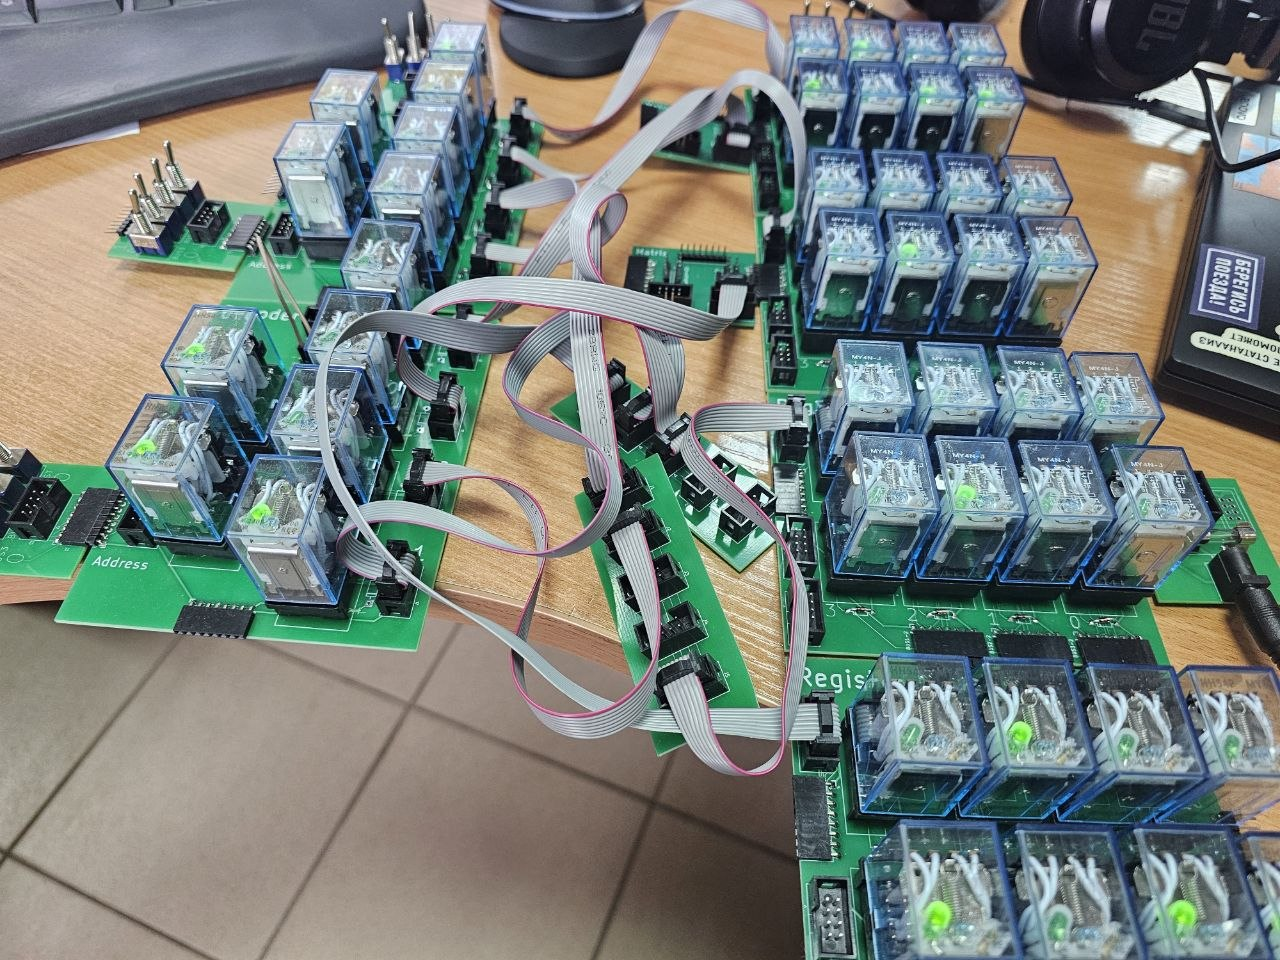
\includegraphics[width=\columnwidth]{photo/register_file2.jpg}

% 2 дешифратора: один для выбора регистра и сброса, второй для выбора второго регистра
% 4 регистра
% 4 шины для подключения сигналов от нескольких источников к каждому регистру
% 4 модуля переключателей: один для выбора управляющих сигналов, два для адресов и один для ввода начальных значений

Проверьте работу собранного регистрового файла:

\begin{itemize}
    \item Установите на входе любого из дешифраторов адрес~$0010$ и выберите регистр на шину с помощью управляющих тумблеров.
    \item Установите на тумблерах, подключённых к шине~$1$ значение~$0110$. Убедитесь, что оно записалось в третий по счёту регистр
          (его адрес как раз и будет $0010$, так как нумерация начинается с нуля).
    \item Сбросьте все тумблеры в $0$.
    \item Установите на входе одного дешифратора адрес $0010$, а на входе другого --- $0011$.
    \item Теперь включите два управляющих бита для выборки регистров ($1$ и $2$). Убедитесь, что третий и четвёртый по счёту
          регистры подключились к шине~$1$. При этом в четвёртый регистр скопируется значение из третьего.
    \item Сбросьте все тумблеры в $0$.
    \item Проделайте аналогичные действия, чтобы сбросить значения регистров. Для этого нужно будет активировать
          бит~$0$ на управляющих тумблерах.
\end{itemize}
